\documentclass[
	% -- opções da classe memoir --
	12pt,				% tamanho da fonte
	openright,			% capítulos começam em pág ímpar (insere página vazia caso preciso)
%	twoside,			% para impressão em recto e verso. Oposto a oneside
	oneside,
	a4paper,			% tamanho do papel.
	% -- opções da classe abntex2 --
	sumario=tradicional,
	chapter=TITLE,		% títulos de capítulos convertidos em letras maiúsculas
	section=TITLE,		% títulos de seções convertidos em letras maiúsculas
	%subsection=TITLE,	% títulos de subseções convertidos em letras maiúsculas
	%subsubsection=TITLE,% títulos de subsubseções convertidos em letras maiúsculas
	% -- opções do pacote babel --
	english,			% idioma adicional para hifenização
	french,				% idioma adicional para hifenização
	spanish,			% idioma adicional para hifenização
	brazil				% o último idioma é o principal do documento
	]{ftex}
% ---
% Pacotes básicos
% ---
\usepackage{lmodern}			% Usa a fonte Latin Modern
\usepackage[T1]{fontenc}		% Selecao de codigos de fonte.
\usepackage[utf8]{inputenc}		% Codificacao do documento (conversão automática dos acentos)
\usepackage{lastpage}			% Usado pela Ficha catalográfica
\usepackage{indentfirst}		% Indenta o primeiro parágrafo de cada seção.
\usepackage{color}				% Controle das cores
\usepackage{graphicx}			% Inclusão de gráficos
\usepackage{microtype} 			% para melhorias de justificação
\usepackage[table]{xcolor}

\usepackage{float}
\usepackage{multirow}
\usepackage[skip=2pt,font=scriptsize]{caption}
\usepackage{nomencl}
\usepackage{subfigure}
\usepackage{pdflscape}
\usepackage{pdfpages}
\usepackage{xcolor}
\usepackage{textgreek}
\usepackage{amsmath}
\usepackage{nccmath}
\usepackage{setspace}
% Definindo novas cores
\definecolor{verde}{rgb}{0.25,0.5,0.35}
\definecolor{jpurple}{rgb}{0.5,0,0.35}
% Configurando layout para mostrar codigos
\usepackage{listings}
\usepackage{chngcntr}
\newcommand{\estiloJava}{
    \lstset{
        language=Java,
        basicstyle=\ttfamily\small,
        keywordstyle=\color{jpurple}\bfseries,
        stringstyle=\color{red},
        commentstyle=\color{verde},
        morecomment=[s][\color{blue}]{/**}{*/},
        showspaces=false,
        showstringspaces=false,
        numbers=left,
        numberstyle=\tiny,
        breaklines=true,
        backgroundcolor=\color{cyan!10},
        breakautoindent=true,
        captionpos=t,
        xleftmargin=0pt,
        columns=fullflexible,
        frame=single,
        frameround=tttt,
        tabsize=2,
        belowskip=-12pt
    }
}
\newcommand{\estiloHtml}{
    \lstset{
        language=HTML,
        basicstyle=\small\ttfamily,
        keywordstyle=\color{black}\bfseries,
        breaklines=true,
        columns=fullflexible,
        frame=single,
        frameround=tttt,
        showstringspaces=false,
        tabsize=2,
    }
}
\renewcommand{\lstlistingname}{Listagem}
\AtBeginDocument{\counterwithout{lstlisting}{section}}
% \usepackage[square,sort]{natbib}
% ---

% ---
% Pacotes adicionais, usados apenas no âmbito do Modelo Canônico do abnteX2
% ---
\usepackage{lipsum}				% para geração de dummy text
% ---

% ---
% Pacotes de citações
% ---
% \usepackage[brazilian,hyperpageref]{backref}	 % Paginas com as citações na bibl
\usepackage[alf,
    versalete,
    abnt-emphasize=bf,
    abnt-etal-list=3,
    abnt-etal-text=it,
    abnt-and-type=&,
    abnt-last-names=abnt,
    abnt-repeated-author-omit=no
]{abntex2cite}	% Citações padrão ABNT

% ---
% CONFIGURAÇÕES DE PACOTES
% ---

% ---
% Configurações do pacote backref
% Usado sem a opção hyperpageref de backref
% \renewcommand{\backrefpagesname}{Citado na(s) página(s):~}
% Texto padrão antes do número das páginas
\renewcommand{\backref}{}
% Define os textos da citação
% \renewcommand*{\backrefalt}[4]{
%	\ifcase #1 %
%		Nenhuma citação no texto.%
%	\or
%		Citado na página #2.%
%	\else
%		Citado #1 vezes nas páginas #2.%
%	\fi}%
% Espaçamento extra nas linhas de tabelas
\renewcommand{\arraystretch}{1.5}
% Fonte Arial
\usepackage{helvet}
\renewcommand{\familydefault}{\sfdefault}
% ---

% ---
% Configurações de aparência do PDF final

% alterando o aspecto da cor azul
\definecolor{blue}{RGB}{41,5,195}

% informações do PDF
\makeatletter
\hypersetup{
     	%pagebackref=true,
		pdftitle={\@title},
		pdfauthor={\@author},
    	pdfsubject={\imprimirpreambulo},
	    pdfcreator={LaTeX with abnTeX2},
		pdfkeywords={abnt}{latex}{abntex}{abntex2}{trabalho acadêmico},
		colorlinks=true,       		% false: boxed links; true: colored links
    	linkcolor=blue,          	% color of internal links
    	citecolor=blue,        		% color of links to bibliography
    	filecolor=magenta,      		% color of file links
		urlcolor=blue,
		bookmarksdepth=4
}
\makeatother
% ---


% ---
% compila o indice
% ---
\makeindex
% ---

% ---
% compila a lista de siglas e abreveaturas
\makenomenclature
% ---

\begin{document}
% Seleciona o idioma do documento (conforme pacotes do babel)
%\selectlanguage{english}
\selectlanguage{brazil}

% Retira espaço extra obsoleto entre as frases.
\frenchspacing

% ----------------------------------------------------------
% ELEMENTOS PRÉ-TEXTUAIS
% ----------------------------------------------------------
\pretextual

% ---
% Capa
% ---
% ---
% Informações de dados para CAPA e FOLHA DE ROSTO
% ---
\titulo{TÍTULO DO TRABALHO}
\autor{FULANO DE TAL}
\local{Caxias do Sul}
\data{2018}
\orientador{Prof. Dr./Mr./Esp. Siclano de Tal}
%\coorientador{}
\instituicao{
\begin{figure}[!ht]
    \centering
    
\includegraphics{img/logo-uniftec-azul-35x877.png}
\end{figure}
CURSO SUPERIOR DE ...}
\tipotrabalho{Trabalho acadêmico}
% O preambulo deve conter o tipo do trabalho, o objetivo,
% o nome da instituição e a área de concentração
\preambulo{Trabalho apresentado para o Curso de ...,
do Centro Universitário Uniftec, como parte dos requisitos para avaliação da unidade curricular de ...}
% ---

\imprimircapa
% ---
% ---

% Folha de rosto
% (o * indica que haverá a ficha bibliográfica)
% ---
\imprimirfolhaderosto*
% ---

\makeatletter
\begin{folhadeaprovacao}
\begin{center}
    {\ABNTEXchapterfont\bfseries\normalsize\imprimirautor}
    \vfill

    \ABNTEXchapterfont\bfseries\large\imprimirtitulo
\end{center}

% \vspace*{\fill}
\vfill

\abntex@ifnotempty{\imprimirpreambulo}{%
  \hspace{.35\textwidth}
  \begin{minipage}{.5\textwidth}
  \ABNTEXchapterfont\bfseries\normalsize\imprimirpreambulo
  \end{minipage}%
%   \vspace*{\fill}
  \vfill
}%
\ABNTEXchapterfont\bfseries\normalsize{}Aprovado em:
\vfill
\begin{center}
    \ABNTEXchapterfont\bfseries\normalsize{}BANCA EXAMINADORA \\
    \assinatura{{\bfseries\normalsize{}Professor Orientador: }}
    \assinatura{{\bfseries\normalsize{}Professor Avaliador: }}
    \assinatura{{\bfseries\normalsize{}Professor Avaliador: }}
    \vspace*{\fill}
    {\bfseries\normalsize\imprimirlocal}
    \par
    {\bfseries\normalsize\imprimirdata}
\end{center}
\end{folhadeaprovacao}
\makeatother


\begin{Spacing}{1.0}

\begin{center}
    \ABNTEXchapterfont\bfseries\large\imprimirtitulo
\end{center}
\hfill

\hspace*{0pt}\hfill \bfseries\normalsize Folano de Tal

\hspace*{0pt}\hfill \normalfont Autor

\hspace*{0pt}\hfill \normalfont folano@gmail.com

\hfill

\hspace*{0pt}\hfill
{\bfseries\normalsize\imprimirorientador\par}

\hspace*{0pt}\hfill \normalfont\normalsize Orientador

\hspace*{0pt}\hfill \normalfont orientador@gmail.com

\hfill

\hfill

\begin{resumo}
    
\textbf{Resumo:}
Template Latex para o modelo FTEC.

\hfill

\textbf{Palavras-chave}:
Template. Latex.
\end{resumo}
\end{Spacing}\PRIVATEclearpageifneeded

% resumo em inglês
\begin{Spacing}{1.0}
    \begin{otherlanguage*}{english}

\begin{center}
    \ABNTEXchapterfont\bfseries\large\imprimirtitulo
\end{center}
\hfill

\hspace*{0pt}\hfill \bfseries\normalsize Folano de Tal

\hspace*{0pt}\hfill \normalfont Autor

\hspace*{0pt}\hfill \normalfont folano@gmail.com

\hfill

\hspace*{0pt}\hfill
{\bfseries\normalsize\imprimirorientador\par}

\hspace*{0pt}\hfill \normalfont\normalsize Orientador

\hspace*{0pt}\hfill \normalfont orientador@gmail.com

\hfill

\hfill

\begin{resumo}[]
    
\textbf{Abstract:}
Latex Template for the FTEC model.

\hfill

\textbf{Keywords}:
Template. Latex.
\end{resumo}
    \end{otherlanguage*}
\end{Spacing}\PRIVATEclearpageifneeded

  
  
% ---
% inserir lista de ilustrações
% ---
\pdfbookmark[0]{\listfigurename}{lof}
\listoffigures*
\cleardoublepage
% ---

% ---
% inserir lista de tabelas
% ---
\pdfbookmark[0]{\listtablename}{lot}
\listoftables*
\cleardoublepage
% ---
 
% ---
% inserir lista de abreviaturas e siglas
% ---
\renewcommand{\nomname}{\listadesiglasname}
\pdfbookmark[0]{\nomname}{las}
% \begin{siglas}
%   \item[API] Application Programming Interface
%   \item[CRUD] Create, Read, Update e Delete
%   \item[MVC] Model View Control
% \end{siglas}
\makenomenclature
\printnomenclature
\cleardoublepage
% ---


% ---
% inserir o sumario
% ---
\pdfbookmark[0]{\contentsname}{toc}
%\dominitoc
\tableofcontents*
\cleardoublepage
% ---

 \captionsetup[table]{
  labelsep = newline,
%   justification=justified,
  justification=centering,
%   font=bf,
  singlelinecheck=false,%%%%%%% a single line is centered by default
  labelsep=colon,%%%%%%
 % skip = \medskipamount
}
  
  
\captionsetup[figure]{
  labelsep=colon,%%%%%%
%   font=bf,
  labelfont=bf,
  justification=centering,
  singlelinecheck=false,%%%%%%% a single line is centered by default
%   skip = \medskipamount
}
  
% ----------------------------------------------------------
% ELEMENTOS TEXTUAIS
% ----------------------------------------------------------
\textual

% ---
% !TEX root = ../main.tex
\chapter{INTRODUÇÂO}

\lipsum[2-10]

\section{Problema}

\lipsum[3-5]

\section{Hipóteses}

\lipsum[5]
\begin{itemize}
    \item Hipótese 1
    \item Hipótese 2
    \item Hipotese n
\end{itemize}

\section{Objetivo geral}

\lipsum[6]

\section{Objetivos Específicos}

\lipsum[7]
\begin{itemize}
    \item Objetivo 1
    \item Objetivo 2
    \item Objetivo n
\end{itemize}

\section{Justificativa}

\lipsum[7-20]

\section{Cronograma de Atividades}

\chapter{Fundamentação teórica}

Sobre a fundamentação teórica, o \citeonline{ftec18} diz o seguinte:

\begin{citacao}
"A fundamentação teórica consiste num levantamento sobre a temática, fornecendo uma visão geral do que já existe escrito sobre o assunto e que serve como base para a investigação prática. Entretanto, todo o texto deve ser escrito com as palavras do autor da monografia ou TCC. As citações complementam, fundamentam e justificam as ideias que estão sendo descritas."
\end{citacao}

\section{Assunto 1}

Para o \citeonline{autorx13}, esse é um exemplo de citação curta.

\lipsum[1-2]

\begin{figure}[!ht]
    \centering
    \caption{Fachada do Uniftec}
    \label{graf1}
    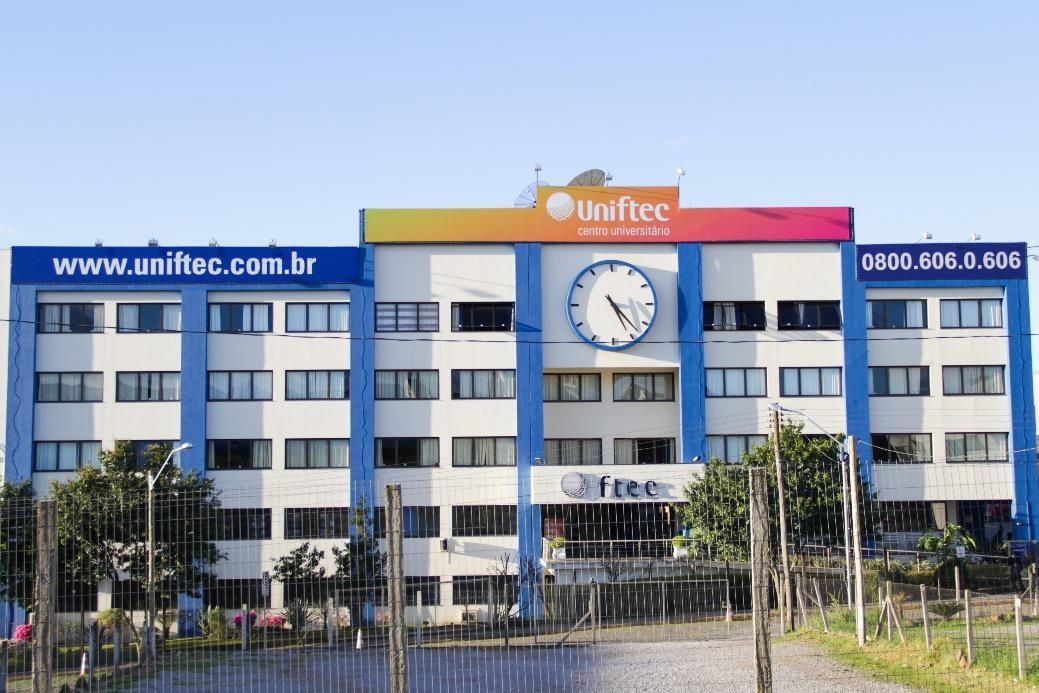
\includegraphics[width=1\textwidth]{img/fachada.jpg}
    \captionsetup{justification=normal}
    \legend{Fonte: Uniftec (2018)}
\end{figure}

\section{Assunto 2}

\lipsum[2-3]

\subsection{Sub assunto}

\lipsum[3-4]

\subsubsection{Sub-sub assunto}

\lipsum[4-5]

\subsubsubsection{Sub-sub-sub assunto}

\lipsum[5-6]

\chapter{Procedimentos metodológicos}

O \citeonline{ftec18} cita que, os procedimentos metodológicos consistem em descrever o seguinte:

\begin{enumerate}[label=\alph*)]
    \item a metodologia utilizada na realização da pesquisa;
    \item a população e/ou objeto investigado; bem como a amostragem;
    \item os procedimentos técnicos empregados na obtenção dos dados, como foram
construídos e utilizados;
    \item a explicitação dos tipos de fontes utilizadas e dados foram coletados; e e) o relato dos diferentes momentos do processo investigativo.
\end{enumerate}

O referido manual, também ressalta que deve ser utilizado o tempo verbal no passado.


\chapter{Apresentação e análise dos resultados}
\chapter{Considerações finais}

\postextual

% ---
% Bibliografia
\bibliography{bibliografia}
% ---

%\include{postextual/apendices}

% ---
% Anexo 1 manual do usuário
% ---

% ---
% Anexo 2 Estratégia de testes
% ---

\end{document}

